\begin{table}[b]
\vspace{-0.1in}
\caption{Considered Connection Statements.}
\label{tbl:connections}
\centering
\tabcolsep=1.5pt
\resizebox{\columnwidth}{!}{%
\begin{tabular}{|l|l|l|l|}
\hline
& \textbf{Class or Interface} & \textbf{Method} & \textbf{Indication of Failure}\\
\hline
 1. & java.net.URL                       & openConnection  & java.io.IOException \\
 2. & java.net.URLConnection             & connect         & java.io.IOException \\
 3. & org.apache.http.client.HttpClient  & execute         & java.io.IOException \\
 4. & java.net.Socket                    & getOutputStream & java.io.IOException \\
% 5. & android.os.IBinder                 & transact        & android.os.RemoteException \\
\hline
\end{tabular}
}%resizebox
%\vspace{-0.1in}
\end{table}



\vspace{-0.1in}
\section{Communication in Android}
\label{sec:study} 

In this section, we describe the design of the study that we conducted to gain more insights into the nature of communication performed by Android applications. We then discuss the study results. 

\subsection{Design of the Study}

%\vspace{0.05in}
%\noindent 
%{\bf Connection Statements.}
\subsubsection{Connection Statements}
The list of the connection statements that we consider in our study is given in Table~\ref{tbl:connections}.
The first three are responsible for establishing HTTP connections with backend servers, with the forth one provides socket-based communication. We also included all classes that derive from those listed in Table~\ref{tbl:connections}.
% and the last one allows 
%RPC communication with other applications and services installed on the same mobile device. 


\begin{table}[t]
\caption{Analyzed Applications.}
\label{tbl:applications}
\centering
\tabcolsep=1.5pt
\resizebox{1\columnwidth}{!}{%
\begin{tabular}{|l|C{0.7cm}|C{1.5cm}|C{1.5cm}|C{1.6cm}|C{1.9cm}|}
\hline
\textbf{Applications} &
\textbf{jar size (MB)} &
\textbf{Total \# of connection statements} &
\textbf{\# of triggered connection statements} &
\textbf{\# of non-essentials\newline(\% of trig.)} &
\textbf{\# of non-essentials in known A\&A\newline(\% of total non-essential)} \\
\hline
%--------------------------------------------------------------------
air.com.sgn.cookiejam.gp   & 2.7  & 17  & 3  & 2 (66.7\%)  & 1 (50.0\%)  \\ % & 1 (33.3\%)  & -
com.crimsonpine.stayinline   & 3.2  & 15  & 2  & 2 (100.0\%)  & 2 (100.0\%)  \\ % & 0 (0.0\%)   & -
com.devuni.flashlight    & 1.4  & 16  & 3  & 1 (33.3\%)  & 1 (100.0\%)  \\ % & 2 (66.7\%)  & -
com.emoji.Smart.Keyboard   & 0.8  & 3   & 3  & 2 (66.7\%)  & 0 (0.0\%)   \\ % & 1 (33.3\%)  & -
com.facebook.katana     & 0.6  & 3   & 0  & -     & -     \\ % & 0 (0.0\%)   & -
com.grillgames.guitarrockhero  & 6.2  & 51  & 14 & 14 (100.0\%)  & 8 (57.1\%)  \\ % & 0 (0.0\%)   & -
com.jb.emoji.gokeyboard    & 5.2  & 42  & 10 & 7 (70.0\%)  & 0 (0.0\%)   \\ % & 3 (30.0\%)  & -
com.king.candycrushsaga    & 2.6  & 15  & 1  & 0 (0.0\%)   & -          \\ % & 1 (100.0\%)  & -
com.pandora.android     & 5.7  & 57  & 12 & 9 (75.0\%)  & 4 (44.4\%)  \\ % & 3 (25.0\%)  & -
com.spotify.music     & 5.4  & 20  & 7  & 3 (42.9\%)  & 1 (33.3\%)  \\ % & 4 (57.1\%)  & -
com.twitter.android     & 5.9  & 21  & 4  & 3 (75.0\%)  & 1 (33.3\%)  \\ % & 1 (25.0\%)  & -
com.walmart.android     & 5.8  & 33  & 8  & 5 (62.5\%)  & 3 (60.0\%)  \\ % & 3 (37.5\%)  & -
net.zedge.android     & 6.5  & 37  & 8  & 4 (50.0\%)  & 4 (100.0\%)  \\ % & 4 (50.0\%)  & -
\hline
%--------------------------------------------------------------------
Total        & 52.0  & 330  & 75 & 52 (69.3\%)   & 25 (48.1\%)  \\ % & 1.8 (30.7\%)  & -
\hline
%--------------------------------------------------------------------
\end{tabular}
}% resizebox
\end{table}


When a connection failure occurs, e.g., when the desired server is unavailable, or when a device is put in the disconnected or airplane mode, each of these methods throws \texttt{java.io.IOException} exception. 
Thus, for investigating the significance of a connection on the overall behavior of an analyzed application, we inject a connection failure by replacing the connection statement with a statement that throw such exception. 
This approach was chosen as it leverages the applications' native mechanism for dealing with failures, thus reducing side-effects introduced by our instrumentation to a minimum.

%\vspace{0.1in}
%\noindent 
%{\bf Application Instrumentation.}
\subsubsection{Application Instrumentation}
As input to our study, we assume an Android application given as an apk file. 
We use the dex2jar tool suite~\cite{dex2jar} to extract the jar file from the apk.
We then use the asm framework~\cite{asm} to implement two types of transformations: 
\begin{enumerate}[leftmargin=0.5cm]%\setlength{\itemsep}{-0.05in}
\item \emph{A monitoring transformation} which produces a version of the original application that logs all executions of the connection statements in Table~\ref{tbl:connections}. 
\item \emph{A blocking transformation} which obtains as additional input a configuration file that specifies the list of connection statements to disable. It then produces a version of the original application in which the specified connection statements are replaced by statements that throw exceptions.
% of the corresponding type, as specified in Table~\ref{tbl:connections}.
\end{enumerate}
The jar file of the transformed application is then converted back to apk using the dex2jar tool suite and signed with the jarsigner tool distributed with the standard Java JDK.
 

%\vspace{0.1in}
%\noindent 
%{\bf Automated Application Execution and Comparison.}
\subsubsection{Automated Application Execution and Comparison}
Comparison of user-observable behavior requires dynamic execution of the analyzed applications. 
The main obstacle in performing such comparison is the ability to reproduce program executions in a repeatable manner. 
To overcome this obstacle, we produce a script that automates the execution of each application.
As the first step, we use the Android getevent tool~\cite{getevent} that runs on the device and captures all user and kernel input events to capture a sequence of events that exercise an application behavior. We make sure to pause between user gestures that assume application response. 
We then enhance the script produced by getevent to insert a screen capturing command after each pause and also between events of any prolonged sequences. 
We upload the produced script onto the device and run it for each version of the application. 

We deliberately opt not to use Android's UI/Application Exerciser Monkey~\cite{monkey} tool. While this tool is able to  
generates a repeatable sequence of pseudo-random streams of events such as clicks, touches and gestures, in our case, 
it was unable to provide a reasonably exhaustive
coverage of application functionality. Even for applications that do not require entering any login credentials, it quickly locked itself out of the application by generating gestures that the analyzed application cannot handle. 
We thus have chosen to manually record the desired application execution scenario, which also included any ``semantic'' user input required by the application, e.g., username and password. 

\begin{figure}[!t]
    \centering
    \subfigure[Screen 1.]{%
    \label{fig:screen1}%
    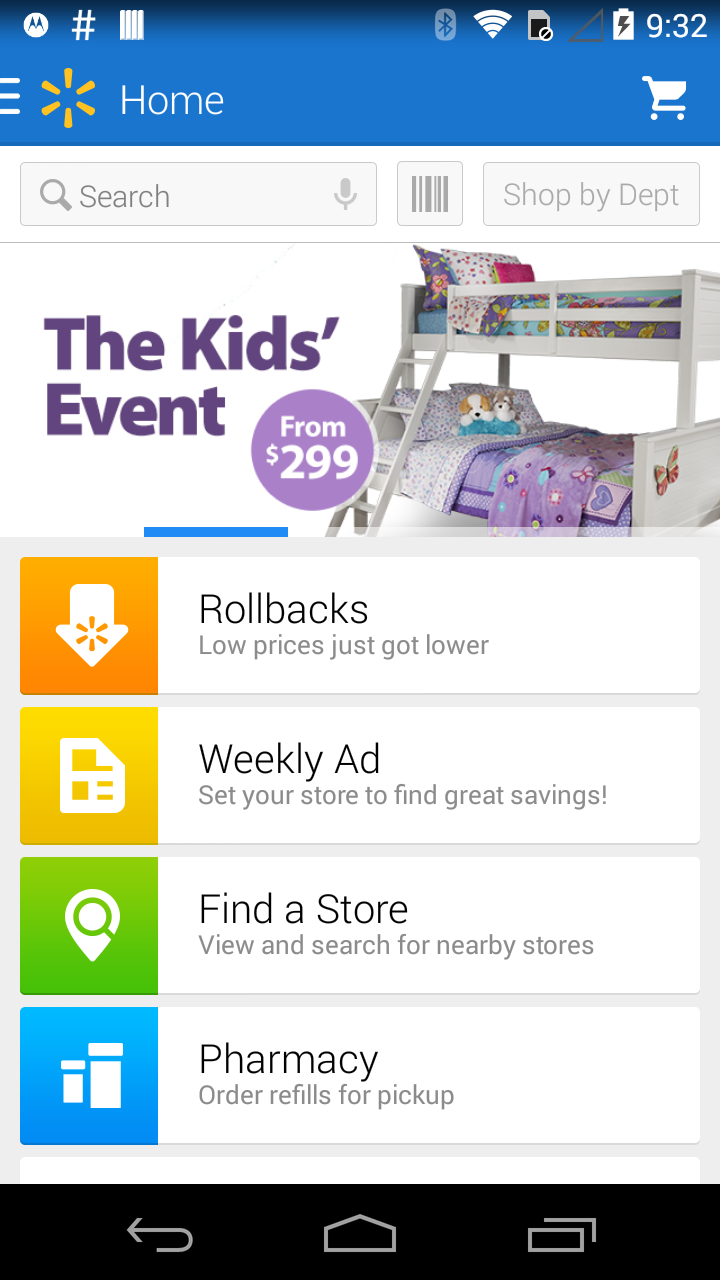
\includegraphics[width=0.3\columnwidth]{img/screen1.png}%
    }
    \hspace{0.5mm}
    \subfigure[Screen 2.]{%
    \label{fig:screen2}%
    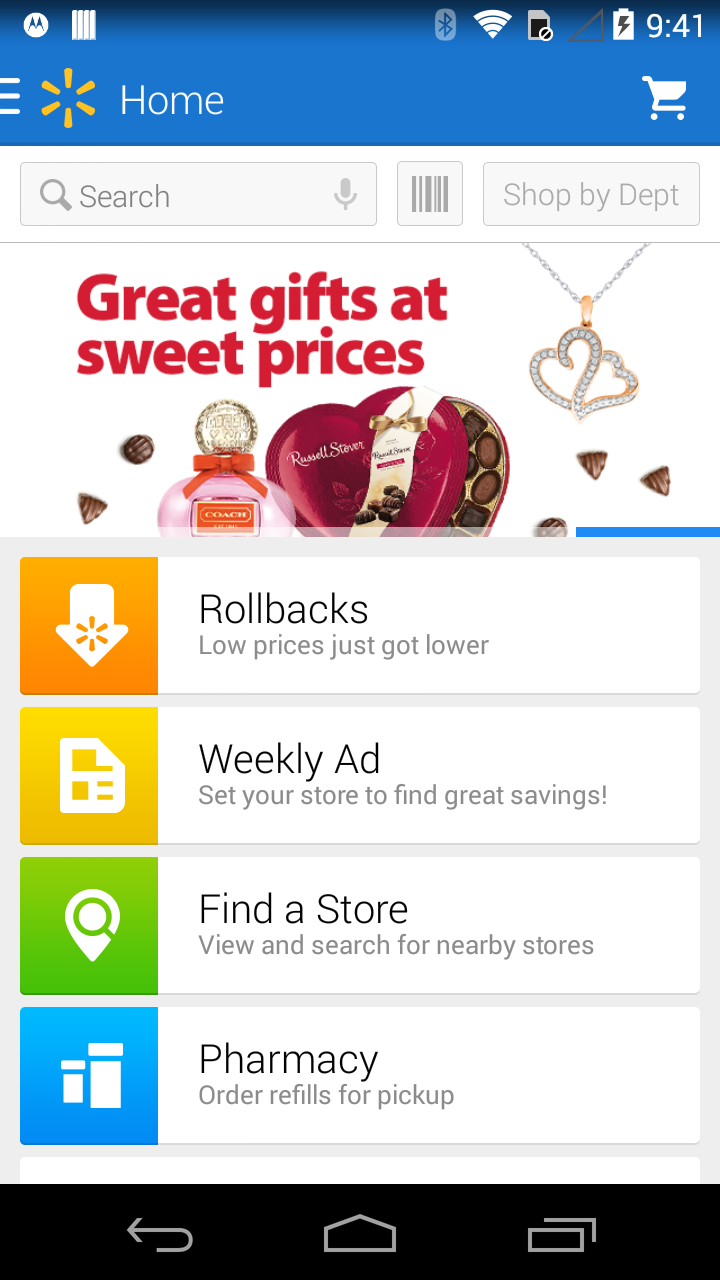
\includegraphics[width=0.3\columnwidth]{img/screen2.png}%
    }
    \hspace{0.5mm}
    \subfigure[Difference for Screens 1 and 2.]{%
    \label{fig:diff12}%
    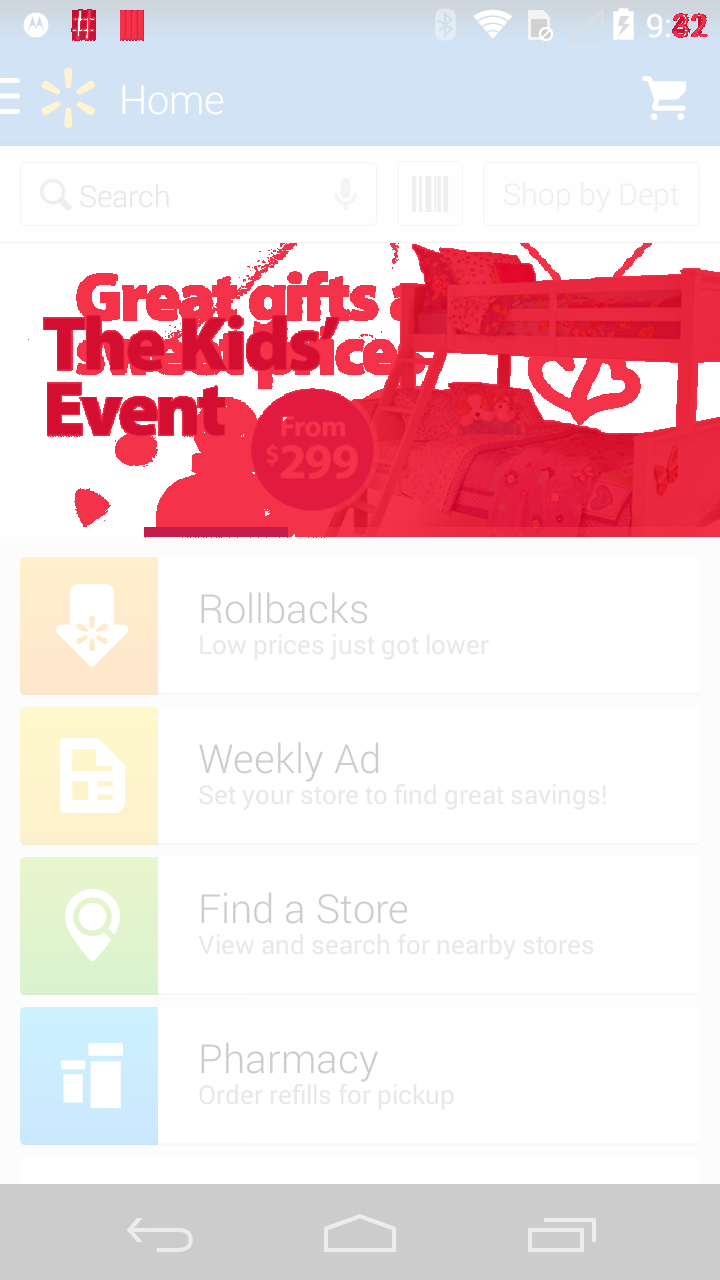
\includegraphics[width=0.3\columnwidth]{img/diff12.png}%
    }%

    \subfigure[Screen 3.]{%
    \label{fig:screen3}%
    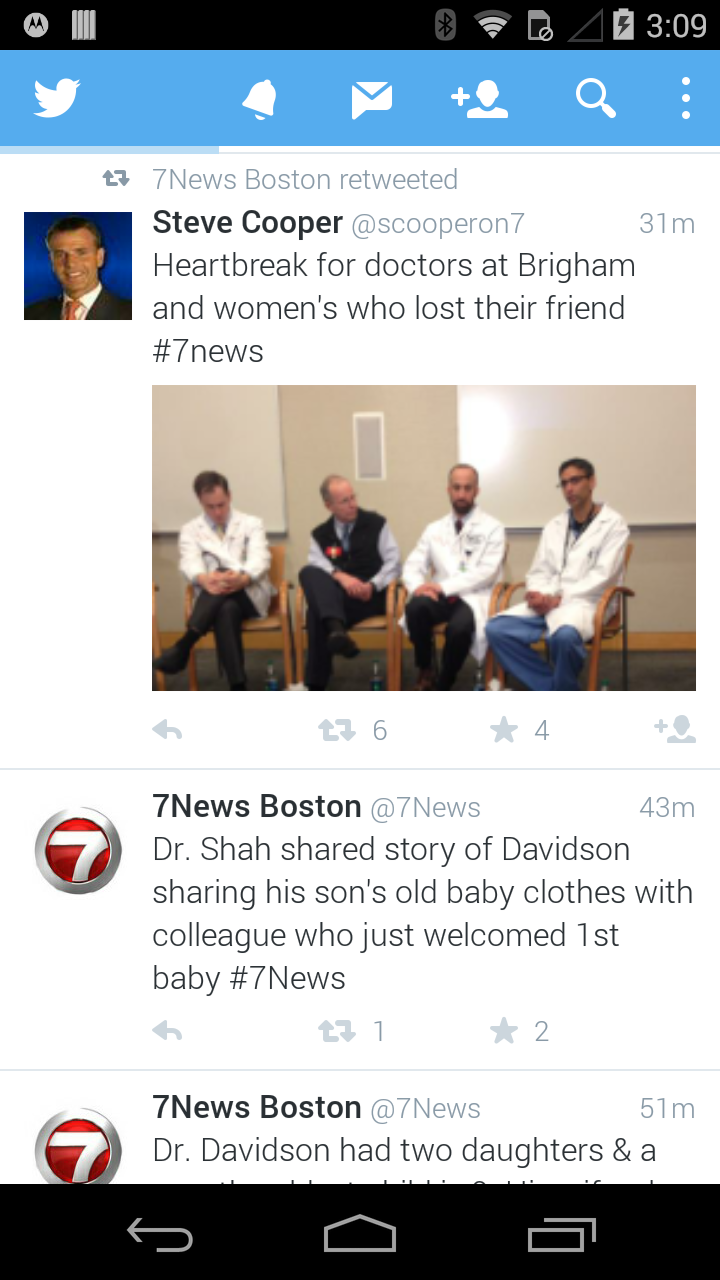
\includegraphics[width=0.3\columnwidth]{img/screen3.png}%
    }
    \hspace{0.5mm}
    \subfigure[Screen 4.]{%
    \label{fig:screen4}%
    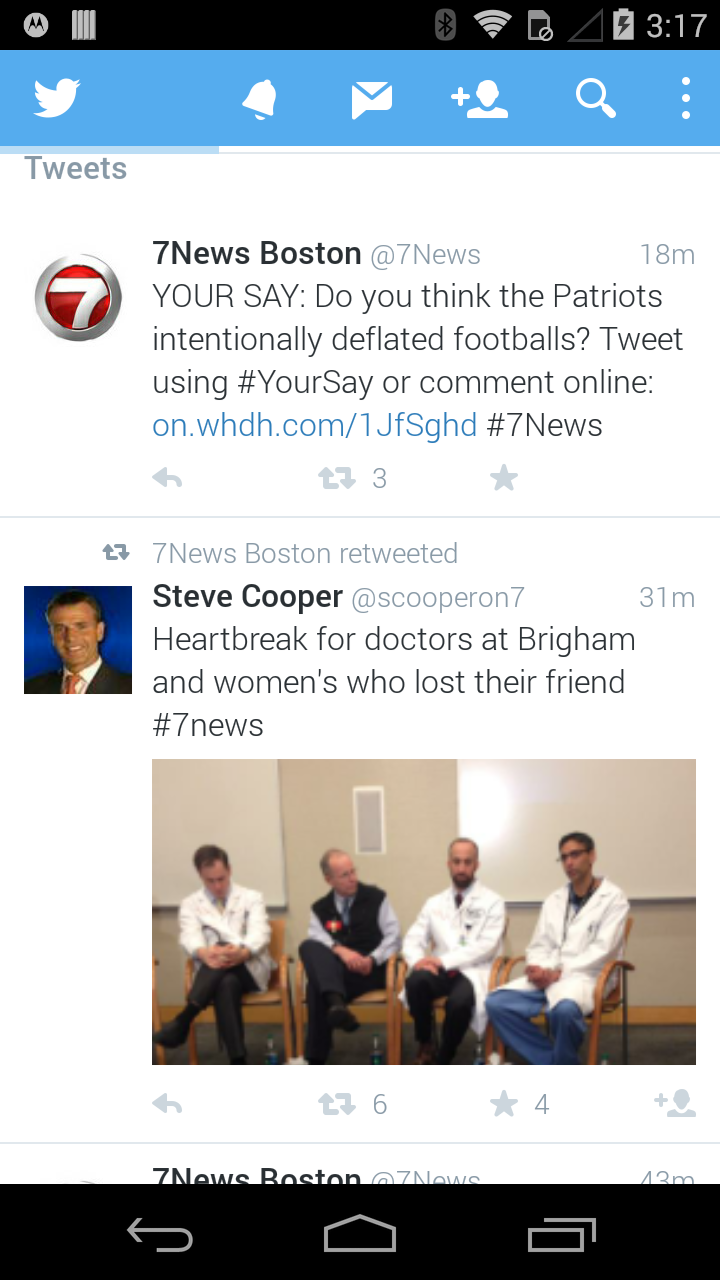
\includegraphics[width=0.3\columnwidth]{img/screen4.png}%
    }
    \hspace{0.5mm}
    \subfigure[Difference for Screens 3 and 4.]{%
    \label{fig:diff34}%
    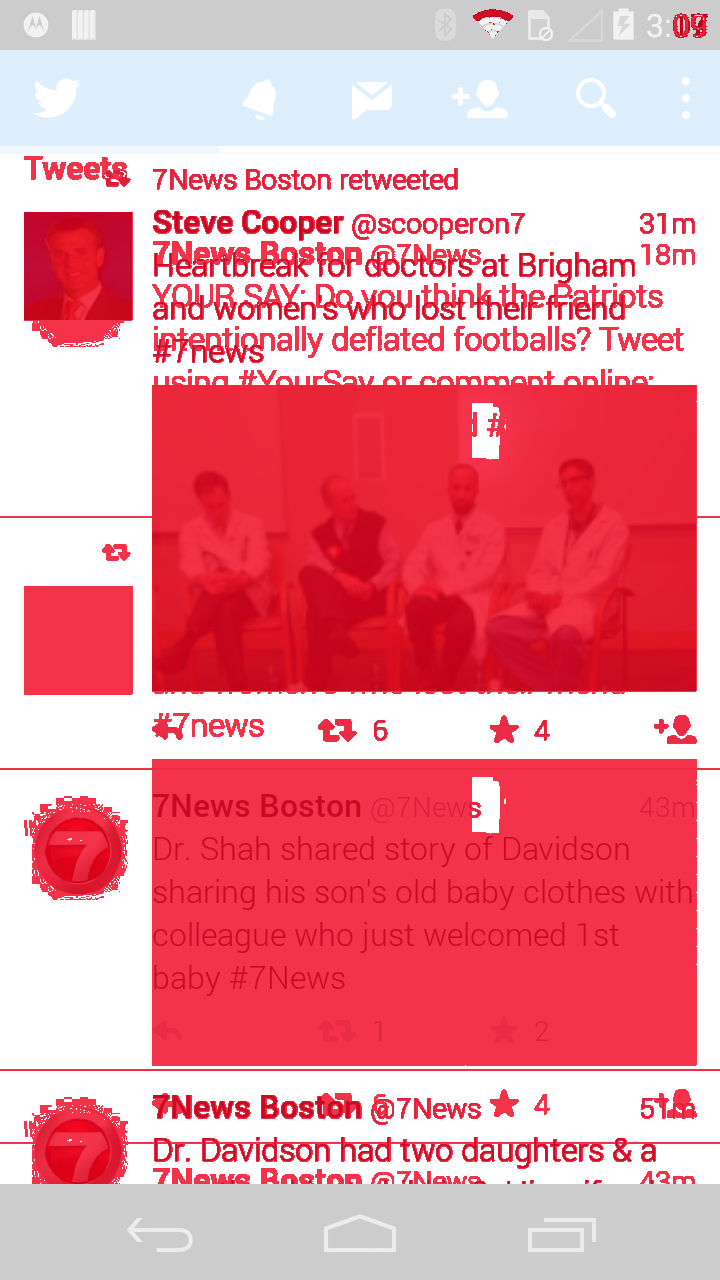
\includegraphics[width=0.3\columnwidth]{img/diff34.png}%
    }
    \caption{Visual differences.}
       \vspace{-0.1in}
    \label{fig:screenshots}
    \vspace{-0.1in}
\end{figure}

For the comparison of application executions, we started by following the approach in~\cite{Hornyack:Han:Jung:Schechter:Wetherall:CCS11}, where screenshots from two different runs are placed side-by-side, 
along with a visual diff of each two corresponding images, as shown in Figure~\ref{fig:screenshots}, for 
the Walmart and twitter applications. 
We used the ImageMagick compare tool~\cite{imagemagick}
to produce the visual diff images automatically. 
We then manually scanned the produced output while ignoring differences in content of advertisement messages and the status of the device, deeming screenshots in Figures~\ref{fig:screenshots}(a) and (b) similar. 
We also ignored the exact content of widgets that are populated by applications in a dynamic manner and are designed to 
provide continuously updated information that is expected to differ between applications runs, such as tweets in Figures~\ref{fig:screenshots}(d) and (e). These two figures are thus also deemed similar.

In one out of the analyzed cases, we had to revert to manual execution and comparison of the application runs.
That case involved interactions with a visual game that required rapid response time, 
thus the automated application execution was unable to provide reliable results. 


%\vspace{0.1in}
%\noindent 
%{\bf Execution Methodology.}
\subsubsection{Execution Methodology}
We performed our study in three phases. In the first phase, we installed the original version of each analyzed 
application on a Nexus 4 mobile device running Android version 4.4.4.
We manually exercised the application for the duration of 5 to 10 minutes, exploring all its functionality visible to us, and recorded the execution script that captured all triggered actions, as described above. 
We then re-installed the application to recreate a ``clean'' initial state and ran the produced execution script.  
We used screenshots collected during this run as the baseline for further comparisons. 

In the second phase, we used the Monitoring Transformation to produce a version of the original application that logs information about all existing and triggered connection statements. We ran the produced version using the execution script and collected the statistics about its communication patterns.  

In the third phase, we iterated over all \emph{triggered} connection statements, disabling them one by one, in order to assess
the necessity of each connection for preserving the user-observable behavior of the application. 
That is, we arranged all triggered connection statements in a list, in a lexical order and then applied the Blocking Transformation to disable the first connection statement in the list.   
We ran the produced version of the application using the recorded execution script and compared the obtained screenshots to the baseline application execution. If disabling the connection statement did not affect the behavior of the application, we marked it as \emph{non-essential}, kept it disabled for the subsequent iterations and proceed to the next connection in the list.
Otherwise, we marked the exercised connection as \emph{essential} and kept it enabled in the subsequent iterations.
We continued with this process until all connections in the list were explored.

%In all iterations, we also disabled all connections that were classified as non-triggered during the second phase. 
%That was done to improve the accuracy 
%of our analysis by proactively preventing applications from taking a new, previously unexplored, path when they detect connection failures. 
As the final quality measure, we manually introspected the execution of the version in which all non-essential connections
were blocked, to detect any  possible issues missed by the automated analysis.

%\vspace{0.1in}
%\noindent 
%{\bf Subjects.} 
\subsubsection{Subjects}
As the subjects of our study, we downloaded 15 top-popular applications available on the Google Play store in November 2014. 
We excluded from this list three chat applications, as our evaluation methodology does not allow assessing the usability of a chat application without a predictably available chat partner. 
We also excluded two applications whose asm-based instrumentation failed, most probably become they use language constructs that are not supported by that framework.

The remaining ten applications are listed in the first column of Table~\ref{tbl:applications}; their corresponding sizes are given in the second column of the table. 
We did not extend our dynamic analysis beyond these ten applications because the inspection of our findings indicated that we reached saturation: while it is clearly infeasible to explore all possible scenarios, we observed similar trends in all analyzed applications. As such, inclusion of additional ones was not expected to provide substantially new insights. 

\subsection{Results}
The quantitative results of the study are presented in columns~3--7 of Table~\ref{tbl:applications}. 
Column 3 and 4 of the table show that only a small number of connection statements encoded in the applications are, in fact, triggered dynamically. 
While some of the non-triggered statements can correspond to execution paths that were not explored during our dynamic application traversal, the vast majority of the statements originate in  
third-party libraries included in the application but only partially used, e.g., various Google services for mobile developers, advertising and analytics libraries and more.
In fact, we identified nine different advertising and analytics libraries used by the ten applications that we analyzed, 
and many times a single applications uses multiple such libraries.

An interesting case is the facebook application (row 3 in Table~\ref{tbl:applications}), where most of the application code is dynamically loaded at runtime from resources shipped within the apk file. 
Our analysis was unable to traverse this dynamically loaded code, and we thus excluded the application from the further analysis, noting that the only three connection statements that existed in the application jar file are never triggered. 

\begin{table}[t]
\caption{Communication Types.}
\label{tbl:statementTypes}
\centering
%\tabcolsep=1.5pt
\resizebox{\columnwidth}{!}{%
\begin{tabular}{|m{3.4cm}|C{2.3cm}|C{1.5cm}|}
\hline
%--------------------------------------------------------------------
                                                &  HTTP and Socket   & RPC \\
\hline
%--------------------------------------------------------------------
    Triggered                                   &  35 (30.7\%)       & 79 (69.3\%) \\
\hline
%--------------------------------------------------------------------
 Non-essential (total)                          &  18 (25.5\%)       & 53 (74.6\%) \\
\hline
%--------------------------------------------------------------------
 Non-essential (Google and Known A\&A Services) & 8 (17.7\%)         & 37 (82.2\%) \\
\hline
%--------------------------------------------------------------------
\end{tabular}
}% resizebox
\vspace{-0.2in}
\end{table}


%\vspace{0.1in}
%\noindent 
%{\bf Classification of the Triggered Statements.}
\subsubsection{Classification of the Triggered Statements}
Column 5 of Table~\ref{tbl:applications} shows the number of connection statements that we determined as non-essential during our study. 
Averaged for all applications, 65\% of the connections fall in that category. 
This means that only 35\% of the connection statements triggered by an application affect its observable behavior, 
when executed for the exact same scenario with the connection being either enabled or disabled (see column 6 of Table~\ref{tbl:applications}). 

Four of the analyzed applications contained advertisement material. For these applications, 71\% of the connections deemed  essential were used for advertising purposes, as shown in the last column of Table~\ref{tbl:applications}.

\conclusion{To answer RQ1, we conclude that non-essential communication often occur in real-world applications: 
65\% of the triggered connection statements can be deemed non-essential.}


Table~\ref{tbl:statementTypes} shows the distribution of the triggered connection statements 
into external communication performed via HTTP and sockets, and internal RPC communication. 
Overall, 30\% of all triggered connection statements correspond to external communication while 70\% -- to
internal ones, as shown in the second row of the table.
The breakdown is similar for the connection statements that we deemed non-essential: slightly more than 25\%
correspond to external communication and the remainder -- to the internal communication with services installed on the same device, as shown in the third row of Table~\ref{tbl:statementTypes}.

The last row of the table present statistic considering the communication with known advertisement and analytic services. The table shows that almost 18\% of the non-essential connections used for these purpose flow to the external services and 82\% -- to internal ones, which further communicate with external services to deliver the required content. 
Google services are commonly, but not exclusively, used by numerous applications. 

%\vspace{0.1in}
%\noindent 
%{\bf Information Leakages.}

%\vspace{0.1in}
%\noindent 
%{\bf Lessons Learned.}
\subsubsection{Lessons Learned}
The collected statistics show that no principle distinction between essential and non-essential connections  
can be made just by considering connection types and their destinations. 
That observation is consistent with findings in~\cite{Hornyack:Han:Jung:Schechter:Wetherall:CCS11}, where authors 
show that blocking all messages to advertising and analytics services made more than 60\% of the applications either less functional or completely dysfunctional. 
We conclude that a more sophisticated 
technique for identifying the non-essential communication performed by the applications is required. 

We manually investigated binaries of several analyzed applications, to gain more insights into the way applications treat non-necessary connections of each of the identified type and communication target. 
We noticed that, in a large number of cases, connection failures are silently ignored by the applications without producing any visual indication to the user. 
That is, the exception triggered by the connection failure of a non-essential connection is either caught and ignored locally in the method that issues the connection or, more commonly, propagated upwards in the call stack and then ignored by one of the calling methods. 

In several cases, an error or warning message is written to the Android log file. However, this file is mostly used by  application developers and is rarely accessed by the end-user.

\conclusion{To answer RQ2, we conjecture that non-essential connections can be detected by inspecting connection failure paths. The lack of updates to GUI elements on the failure path is indicative for a connection being silently ignored by the application, thus being non-essential for the application execution.}










